\documentclass[12pt,a4paper]{report}

% ─── Packages ─────────────────────────────────────────────────────────────────
\usepackage[a4paper, top=2.5cm, bottom=2.5cm, left=3cm, right=2.5cm]{geometry}
\usepackage{graphicx}
\usepackage{amsmath, amssymb}
\usepackage{booktabs}
\usepackage{longtable}
\usepackage{array}
\usepackage{xcolor}
\usepackage{listings}
\usepackage{hyperref}
\usepackage{fancyhdr}
\usepackage{titlesec}
\usepackage{setspace}
\usepackage{caption}
\usepackage{float}
\usepackage{enumitem}
\usepackage{tocloft}
\usepackage{tikz}
\usetikzlibrary{shapes.geometric, arrows.meta, positioning}

% ─── Hyperref Setup ────────────────────────────────────────────────────────────
\hypersetup{
    colorlinks=true,
    linkcolor=blue!60!black,
    urlcolor=blue,
    citecolor=blue,
    pdfauthor={NIT Patna - CSE},
    pdftitle={Real-Time PPE Detection and Safety Compliance Monitoring}
}

% ─── Code Listing Style ────────────────────────────────────────────────────────
\lstdefinestyle{pythonstyle}{
    language=Python,
    backgroundcolor=\color{gray!8},
    basicstyle=\ttfamily\footnotesize,
    keywordstyle=\bfseries\color{blue!70!black},
    commentstyle=\itshape\color{green!50!black},
    stringstyle=\color{red!60!black},
    numbers=left,
    numberstyle=\tiny\color{gray},
    stepnumber=1,
    numbersep=8pt,
    frame=single,
    framerule=0.5pt,
    rulecolor=\color{gray!40},
    breaklines=true,
    breakatwhitespace=true,
    tabsize=4,
    showstringspaces=false,
    captionpos=b
}
\lstset{style=pythonstyle}

% ─── Header / Footer ──────────────────────────────────────────────────────────
\pagestyle{fancy}
\fancyhf{}
\fancyhead[L]{\small\textit{Real-Time PPE Detection \& Safety Compliance Monitoring}}
\fancyhead[R]{\small\textit{NIT Patna --- CSE}}
\fancyfoot[C]{\thepage}
\renewcommand{\headrulewidth}{0.4pt}

% ─── Chapter Title Formatting ─────────────────────────────────────────────────
\titleformat{\chapter}[display]
  {\normalfont\Large\bfseries\centering}
  {\chaptertitlename\ \thechapter}{10pt}{\Large}
\titlespacing*{\chapter}{0pt}{20pt}{25pt}

% ─── Line Spacing ─────────────────────────────────────────────────────────────
\onehalfspacing

% ══════════════════════════════════════════════════════════════════════════════
\begin{document}

% ─── COVER PAGE ───────────────────────────────────────────────────────────────
\begin{titlepage}
\centering

% Institute Logo

\includegraphics[width=3.2cm]{assets/logo.png}\\[0.6cm]

{\LARGE\bfseries National Institute of Technology Patna}\\[0.3cm]
{\large Course: Applied Deep Learning \quad (CS6XXXX)}\\[1.2cm]

\rule{\linewidth}{1.5pt}\\[0.5cm]
{\Huge\bfseries Real-Time PPE Detection and\\[0.3cm] Safety Compliance Monitoring\\[0.2cm] Using Deep Learning}\\[0.4cm]
\rule{\linewidth}{1.5pt}\\[0.6cm]

{\large\itshape Design and implementation of an automated computer vision system using YOLOv8 and PyTorch to monitor workplace safety gear and log compliance violations in real time.}\\[1.2cm]

% Team Table
\begin{tabular}{|p{7cm}|p{4cm}|}
\hline
\textbf{Name} & \textbf{Roll Number} \\
\hline
{[}Enter Team Member 1 Name{]} & {[}Roll No.{]} \\
\hline
{[}Enter Team Member 2 Name{]} & {[}Roll No.{]} \\
\hline
{[}Enter Team Member 3 Name{]} & {[}Roll No.{]} \\
\hline
{[}Enter Team Member 4 Name{]} & {[}Roll No.{]} \\
\hline
Alok Singh & {[}Roll No.{]} \\
\hline
\end{tabular}\\[1.2cm]

{\large Submitted to}\\[0.3cm]
{\large\bfseries {[}Enter Faculty Name{]}}\\[1.0cm]

{\large Department of Computer Science and Engineering}\\[0.2cm]
{\large National Institute of Technology Patna}\\[0.6cm]
{\large\bfseries November 2026}

\end{titlepage}

% ─── TABLE OF CONTENTS ────────────────────────────────────────────────────────
\tableofcontents
\thispagestyle{fancy}
\newpage

% ══════════════════════════════════════════════════════════════════════════════
%  CHAPTER 1 — INTRODUCTION
% ══════════════════════════════════════════════════════════════════════════════
\chapter{Introduction}

\section{Motivation and Significance}

Construction and industrial worksites are among the most hazardous working environments in the world. According to the International Labour Organization (ILO), over 2.3 million workers die each year due to occupational accidents and work-related diseases. A significant proportion of these fatalities and injuries occur as a direct result of workers failing to wear mandatory Personal Protective Equipment (PPE) such as safety helmets (hardhats), high-visibility reflective vests, and face masks.

Traditional worksite safety monitoring relies entirely on manual supervision — safety officers must physically walk the site, observe every worker individually, and issue warnings when non-compliance is observed. This approach is not only resource-intensive and expensive but is fundamentally incapable of providing continuous, uninterrupted monitoring across large construction sites with many workers in different zones simultaneously.

The emergence of \textbf{Deep Learning} and \textbf{Real-Time Computer Vision} presents a transformative opportunity to automate and augment worksite safety enforcement. Modern object detection models, particularly the \textbf{Ultralytics YOLOv8} architecture, can process video streams at high frame rates with remarkable accuracy, detecting both people and their safety gear even under challenging lighting, partial occlusion, and varied camera angles.

This project, \textit{Real-Time PPE Detection and Safety Compliance Monitoring Using Deep Learning}, addresses this critical safety gap by designing and implementing a fully automated, end-to-end PPE monitoring system that:
\begin{itemize}
    \item Detects workers in real-time from video streams, uploaded footage, or live webcam feeds using YOLOv8.
    \item Evaluates whether each detected worker is wearing the required PPE items (Safety Helmet and High-Visibility Safety Vest) using a dual-layer compliance engine combining a dedicated PPE model and calibrated HSV chromatic analysis.
    \item Displays color-coded bounding box annotations — \textcolor{green}{\textbf{green}} for compliant workers and \textcolor{red}{\textbf{red}} for safety violations — alongside an informative HUD banner.
    \item Maintains persistent worker identities across video frames using an IoU-based tracking algorithm with temporal smoothing.
    \item Logs every timestamped violation event, captures snapshot images of violating workers, and provides exportable CSV audit reports through a Streamlit web dashboard.
\end{itemize}

The system is designed to serve as an intelligent, always-on safety compliance assistant that can be deployed in construction, manufacturing, mining, and any regulated industrial environment.

\section{Report Structure}

This report is organized into eight chapters as follows:

\begin{itemize}
    \item \textbf{Chapter 1 — Introduction:} Establishes the motivation, significance, and overview of the project.
    \item \textbf{Chapter 2 — Theoretical Background:} Covers the deep learning and computer vision concepts underlying the system, including YOLOv8 architecture details.
    \item \textbf{Chapter 3 — System Architecture and Design:} Describes the overall system design, the PPE compliance engine, and the real-time processing pipeline.
    \item \textbf{Chapter 4 — Implementation Details:} Explains the actual Python code modules and key implementation decisions.
    \item \textbf{Chapter 5 — How to Run the Project:} Step-by-step instructions for setting up and running the application.
    \item \textbf{Chapter 6 — Testing and Evaluation:} Presents experimental results with test cases and performance observations.
    \item \textbf{Chapter 7 — Limitations and Future Enhancements:} Discusses current limitations and proposes future improvements.
    \item \textbf{Chapter 8 — Conclusion:} Summarizes the contributions and outcomes of the project.
\end{itemize}

% ══════════════════════════════════════════════════════════════════════════════
%  CHAPTER 2 — THEORETICAL BACKGROUND
% ══════════════════════════════════════════════════════════════════════════════
\chapter{Theoretical Background}

\section{Deep Learning \& Computer Vision Building Blocks}

\subsection*{Convolutional Neural Networks (CNNs)}
The foundation of modern computer vision systems is the \textbf{Convolutional Neural Network (CNN)}. CNNs learn spatial hierarchies of visual features — from low-level edges and color gradients in early layers to high-level semantic representations such as ``helmet-shaped object'' or ``reflective vest'' in deeper layers. This hierarchical feature learning makes CNNs particularly effective for detecting objects in natural images.

\subsection*{Object Detection}
Object detection is the task of simultaneously identifying the \textit{class} and \textit{location} (bounding box) of one or more objects within an image. This project requires object detection at two levels: (1) detecting the presence and location of people (workers), and (2) detecting PPE items on each worker's body.

\subsection*{HSV Color Space Analysis}
The Hue-Saturation-Value (HSV) color model separates chromatic information (Hue) from intensity (Value), making it far more robust than RGB for color-based segmentation under varying illumination. This project exploits HSV analysis to verify the presence of fluorescent safety vests (neon lime-green: H $\in$ [13, 34]) and yellow/amber hardhats (H $\in$ [14, 36]) directly from the pixel distribution of worker body region crops.

\subsection*{Non-Maximum Suppression (NMS)}
In object detection, multiple overlapping bounding boxes may be predicted for the same object. Non-Maximum Suppression (NMS) selects the box with the highest confidence score and suppresses all other boxes whose Intersection over Union (IoU) with the selected box exceeds a threshold $\tau$:
\[
\text{IoU}(B_1, B_2) = \frac{|B_1 \cap B_2|}{|B_1 \cup B_2|}
\]
In this project, $\tau = 0.45$ is used as the default IoU threshold for NMS.

\section{Core Technologies}

\subsection{PyTorch Tensor Engine}
PyTorch is the deep learning framework underpinning this project. All model inference operations — forward passes through YOLOv8's convolutional layers — are executed as PyTorch tensor computations. When a GPU is available, tensors are allocated on CUDA devices for massively accelerated parallel computation. The project uses \texttt{torch 2.x} for model loading, inference, and result extraction via \texttt{boxes.xyxy.cpu().numpy()}.

\subsection{Ultralytics YOLOv8 Architecture}

\textbf{YOLO (You Only Look Once)} is a family of real-time object detection architectures that predict bounding boxes and class probabilities in a single neural network forward pass. YOLOv8, developed by Ultralytics (2023), is the latest generation offering superior speed-accuracy trade-offs.

\subsubsection*{CSPDarknet Backbone}
The backbone is responsible for extracting rich visual features from the input image. YOLOv8 uses a \textbf{CSPDarknet} (Cross-Stage Partial Darknet) backbone incorporating C2f (Cross-Stage Partial with two bottlenecks) modules. These modules improve gradient flow and feature re-use, enabling deeper and more expressive feature hierarchies without proportional increases in computation.

\subsubsection*{PANet Neck}
The \textbf{Path Aggregation Network (PANet)} neck bridges the backbone and detection head by aggregating multi-scale feature maps. It combines:
\begin{itemize}
    \item \textbf{Top-down FPN path}: propagates high-level semantic information down to smaller-scale feature maps.
    \item \textbf{Bottom-up PAN path}: propagates precise low-level localization information upward.
\end{itemize}
This bidirectional aggregation allows YOLOv8 to simultaneously detect large objects (a person seen from far away) and small objects (a hardhat on a distant worker).

\subsubsection*{Anchor-Free Detection Head}
Unlike previous YOLO versions that relied on predefined anchor boxes, YOLOv8 uses an \textbf{anchor-free} detection head. It decouples the classification and regression branches:
\begin{itemize}
    \item The \textbf{classification branch} predicts the probability distribution over classes at each spatial location.
    \item The \textbf{regression branch} directly predicts the four coordinates of the bounding box $(x_1, y_1, x_2, y_2)$ using Distribution Focal Loss (DFL).
\end{itemize}
This design reduces the number of hyperparameters and improves generalization across diverse object scales and aspect ratios.

\subsubsection*{Non-Maximum Suppression (NMS) Post-Processing}
After the detection head produces raw predictions, NMS filters redundant overlapping boxes. The IoU threshold $\tau = 0.45$ and confidence threshold $p = 0.30$ are used in this project.

\subsection{OpenCV (Open Source Computer Vision Library)}
OpenCV 4.x is used throughout this project for:
\begin{itemize}
    \item \textbf{Video I/O}: \texttt{cv2.VideoCapture()} reads frames from video files and webcams.
    \item \textbf{Frame Resizing}: High-resolution 4K frames ($3840 \times 2160$) are dynamically downscaled to 1080p for real-time inference.
    \item \textbf{HSV Conversion}: \texttt{cv2.cvtColor(frame, cv2.COLOR\_BGR2HSV)} transforms frames for color-based gear verification.
    \item \textbf{Color Masking}: \texttt{cv2.inRange()} segments pixels matching safety gear color ranges.
    \item \textbf{Annotation Drawing}: \texttt{cv2.rectangle()}, \texttt{cv2.putText()}, and \texttt{cv2.addWeighted()} render bounding boxes, labels, and the HUD overlay.
    \item \textbf{Video Export}: \texttt{cv2.VideoWriter()} exports annotated output video files.
\end{itemize}

\subsection{Streamlit Web Framework}
Streamlit transforms Python scripts into interactive web dashboards without requiring any front-end web development skills. In this project, Streamlit provides:
\begin{itemize}
    \item \texttt{st.set\_page\_config()} --- Configures page title, icon, and layout.
    \item \texttt{st.sidebar} --- Houses all configuration controls (input source selector, compliance rule toggles, sensitivity sliders).
    \item \texttt{st.radio()}, \texttt{st.checkbox()}, \texttt{st.slider()} --- Interactive input widgets.
    \item \texttt{st.image()} --- Renders the annotated video frame in real-time.
    \item \texttt{st.metric()} --- Displays live KPI values (Total Workers, Compliant, Violations, Compliance Rate).
    \item \texttt{st.dataframe()} and \texttt{st.download\_button()} --- Shows the violation log table and enables CSV download.
    \item \texttt{st.tabs()} --- Separates the Live Monitoring Feed from the Violation Audit Log.
    \item \texttt{@st.cache\_resource} --- Caches the YOLO model in memory across reruns for performance.
\end{itemize}

% ══════════════════════════════════════════════════════════════════════════════
%  CHAPTER 3 — SYSTEM ARCHITECTURE AND DESIGN
% ══════════════════════════════════════════════════════════════════════════════
\chapter{System Architecture and Design}

\section{PPE Detection \& Compliance Engine}

The system is organized into five tightly integrated Python modules:

\begin{center}
\renewcommand{\arraystretch}{1.4}
\begin{tabular}{|p{3.2cm}|p{8.5cm}|}
\hline
\textbf{Module} & \textbf{Responsibility} \\
\hline
\texttt{config.py} & Global configuration: file paths, HSV color constants, compliance rule defaults, YOLOv8 model paths. \\
\hline
\texttt{detector.py} & Core PPE detection engine. Loads YOLOv8 models, runs inference, performs HSV gear verification, evaluates compliance rules. \\
\hline
\texttt{tracker.py} & IoU-based multi-worker identity tracking with temporal smoothing (sliding-window majority vote). \\
\hline
\texttt{visualizer.py} & Renders HUD banner, color-coded bounding boxes, gear sub-boxes, and compliance labels on frames. \\
\hline
\texttt{app.py} & Streamlit web application: manages UI, session state, video I/O loop, violation logging, CSV export, and snapshot capture. \\
\hline
\end{tabular}
\end{center}

\subsection*{Dual-Layer Compliance Verification}
The compliance engine uses two complementary layers:

\begin{enumerate}
    \item \textbf{Layer 1 — Dedicated PPE Model}: The fine-tuned \texttt{ppe\_yolov8.pt} model (22 MB, trained on the Keremberke protective equipment dataset, 10 classes: \textit{helmet, no\_helmet, mask, no\_mask, glove, no\_glove, goggles, no\_goggles, shoes, no\_shoes}) is run on each individual person crop to detect PPE items.
    \item \textbf{Layer 2 — HSV Chromatic Analysis}: When the PPE model produces no detection, the \texttt{\_check\_gear\_in\_region\_hsv()} function performs region-specific color segmentation on the person's head region (top 25\% of bounding box) for helmets and torso region (18\%--65\%) for vests.
\end{enumerate}

This dual-layer design provides robustness: the neural model excels at close-up, well-lit scenes while the HSV fallback handles distant workers where the PPE model's resolution is insufficient.

\section{Real-Time Frame Processing Flowchart}

\begin{center}
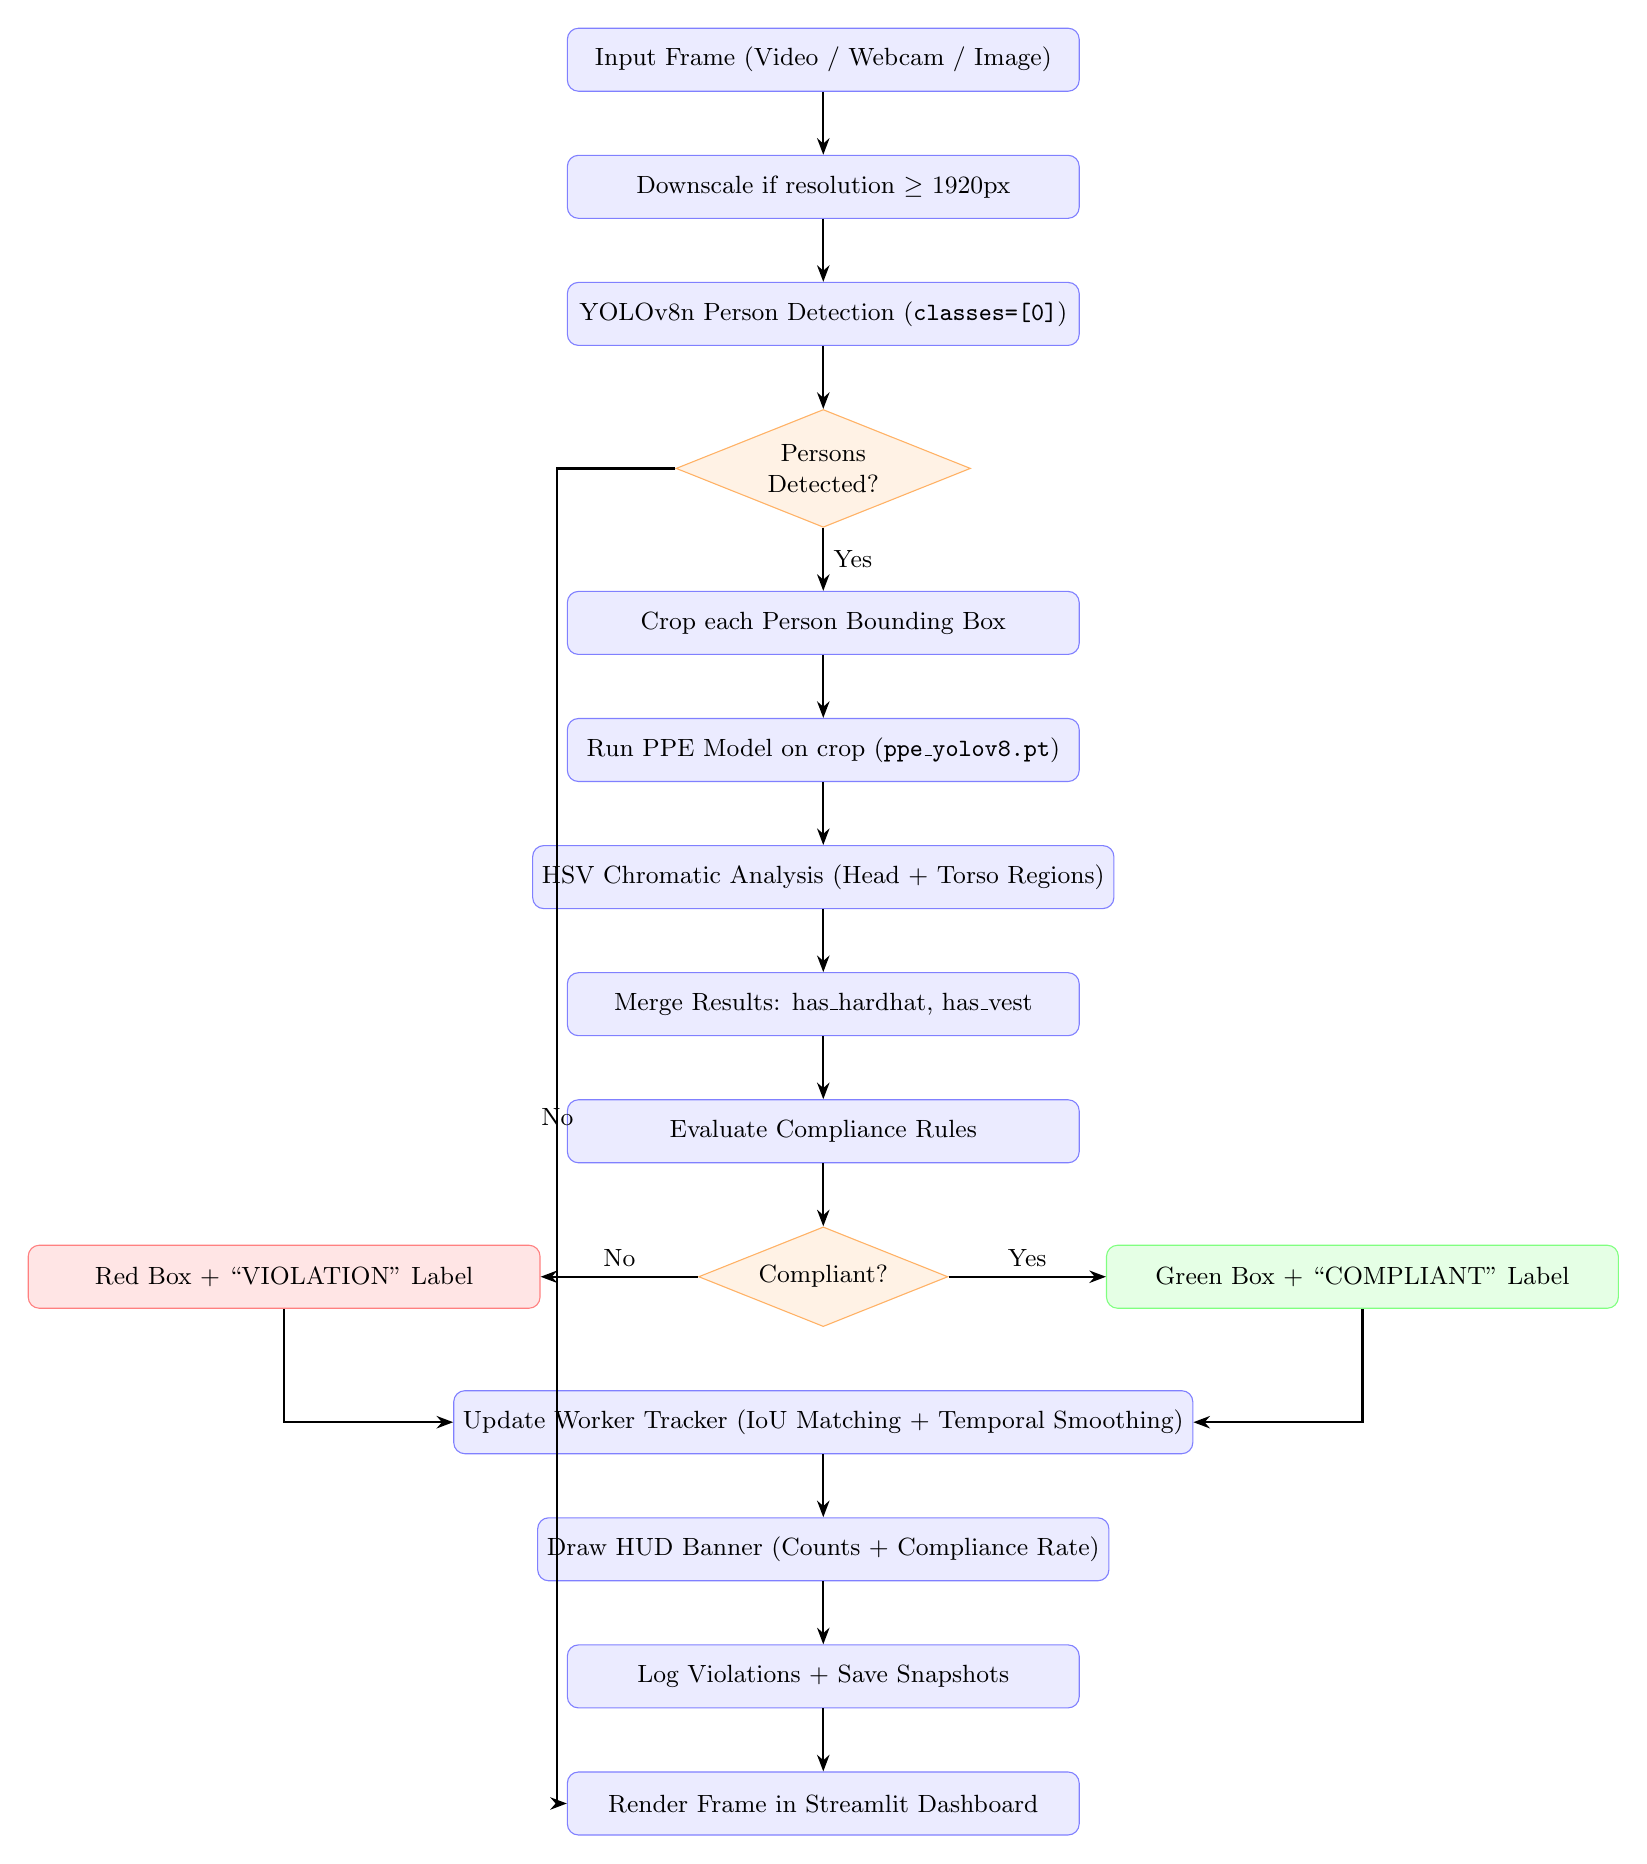
\begin{tikzpicture}[
  node distance = 0.8cm and 0cm,
  box/.style = {rectangle, draw, rounded corners=4pt, minimum width=6.5cm,
                minimum height=0.8cm, align=center, font=\small,
                fill=blue!8, draw=blue!50},
  decision/.style = {diamond, draw, aspect=2.5, fill=orange!10,
                     draw=orange!60, align=center, font=\small},
  arrow/.style = {-{Stealth[length=6pt]}, thick},
  greenbox/.style = {box, fill=green!10, draw=green!50},
  redbox/.style = {box, fill=red!10, draw=red!50},
]

\node[box]       (inp)    {Input Frame (Video / Webcam / Image)};
\node[box, below=of inp]  (resize)  {Downscale if resolution $\geq$ 1920px};
\node[box, below=of resize](yolo)   {YOLOv8n Person Detection (\texttt{classes=[0]})};
\node[decision, below=of yolo](persons) {Persons\\Detected?};
\node[box, below=of persons](crop)  {Crop each Person Bounding Box};
\node[box, below=of crop]  (ppemod) {Run PPE Model on crop (\texttt{ppe\_yolov8.pt})};
\node[box, below=of ppemod](hsv)    {HSV Chromatic Analysis (Head + Torso Regions)};
\node[box, below=of hsv]   (merge)  {Merge Results: has\_hardhat, has\_vest};
\node[box, below=of merge] (rules)  {Evaluate Compliance Rules};
\node[decision, below=of rules](comp) {Compliant?};
\node[greenbox, right=2cm of comp]  (green) {Green Box + ``COMPLIANT'' Label};
\node[redbox,  left=2cm of comp]   (red)   {Red Box + ``VIOLATION'' Label};
\node[box, below=of comp]  (track)  {Update Worker Tracker (IoU Matching + Temporal Smoothing)};
\node[box, below=of track] (hud)    {Draw HUD Banner (Counts + Compliance Rate)};
\node[box, below=of hud]   (log)    {Log Violations + Save Snapshots};
\node[box, below=of log]   (disp)   {Render Frame in Streamlit Dashboard};

\draw[arrow] (inp)     -- (resize);
\draw[arrow] (resize)  -- (yolo);
\draw[arrow] (yolo)    -- (persons);
\draw[arrow] (persons) -- node[right]{\small Yes} (crop);
\draw[arrow] (persons.west) -- ++(-1.5,0) |- node[near start,above]{\small No} (disp);
\draw[arrow] (crop)    -- (ppemod);
\draw[arrow] (ppemod)  -- (hsv);
\draw[arrow] (hsv)     -- (merge);
\draw[arrow] (merge)   -- (rules);
\draw[arrow] (rules)   -- (comp);
\draw[arrow] (comp)    -- node[above]{\small Yes} (green);
\draw[arrow] (comp)    -- node[above]{\small No}  (red);
\draw[arrow] (green.south) |- (track.east);
\draw[arrow] (red.south)   |- (track.west);
\draw[arrow] (track)   -- (hud);
\draw[arrow] (hud)     -- (log);
\draw[arrow] (log)     -- (disp);

\end{tikzpicture}
\end{center}

% ══════════════════════════════════════════════════════════════════════════════
%  CHAPTER 4 — IMPLEMENTATION DETAILS
% ══════════════════════════════════════════════════════════════════════════════
\chapter{Implementation Details}

\section{Code Explanation}

\subsection*{\texttt{detector.py} — PPEDetector Class}

The \texttt{PPEDetector} class is the central intelligence of the system. Its constructor initializes two YOLO models:

\begin{lstlisting}[caption={PPEDetector class initialization (detector.py)}]
class PPEDetector:
    def __init__(self, model_path=None, conf_threshold=0.30,
                 iou_threshold=0.45):
        self.conf_threshold = conf_threshold
        self.iou_threshold  = iou_threshold
        self.person_model   = self._load_person_model()
        self.ppe_model      = self._load_ppe_model()
\end{lstlisting}

The \texttt{detect()} method is the primary inference function. It dynamically adapts the YOLO inference size based on input resolution:

\begin{lstlisting}[caption={Adaptive inference size selection (detector.py)}]
imgsz = 1280 if max(orig_h, orig_w) >= 1920 else 640
res = self.person_model(
    frame, imgsz=imgsz, conf=self.conf_threshold,
    iou=self.iou_threshold, classes=[0], verbose=False
)[0]
\end{lstlisting}

The HSV compliance verification function \texttt{\_check\_gear\_in\_region\_hsv()} segments the person crop into spatial zones:

\begin{lstlisting}[caption={HSV Helmet detection in head region (detector.py)}]
head_h    = max(15, int(h * 0.25))
head_crop = person_crop[0:head_h, :]
head_hsv  = cv2.cvtColor(head_crop, cv2.COLOR_BGR2HSV)
# Yellow hardhat: H in [14,36], S in [70,255], V in [140,255]
yellow_hat_mask  = cv2.inRange(head_hsv,
                    np.array([14, 70,  140]),
                    np.array([36, 255, 255]))
yellow_ratio = cv2.countNonZero(yellow_hat_mask) / head_pixels
has_hardhat  = (yellow_ratio > 0.07) or (white_ratio > 0.18) \
               or (blue_ratio > 0.08)
\end{lstlisting}

\begin{lstlisting}[caption={HSV Safety Vest detection in torso region (detector.py)}]
torso_y1   = int(h * 0.18)
torso_y2   = int(h * 0.65)
torso_crop = person_crop[torso_y1:torso_y2, :]
torso_hsv  = cv2.cvtColor(torso_crop, cv2.COLOR_BGR2HSV)
# Neon lime vest: H in [13,34], S in [60,255], V in [155,255]
neon_vest_mask = cv2.inRange(torso_hsv,
                    np.array([13,  60, 155]),
                    np.array([34, 255, 255]))
neon_ratio = cv2.countNonZero(neon_vest_mask) / torso_pixels
has_vest   = (neon_ratio > 0.08) or (orange_ratio > 0.09)
\end{lstlisting}

\subsection*{\texttt{tracker.py} — WorkerTracker Class}

The \texttt{WorkerTracker} assigns persistent identities to workers using greedy IoU-based bipartite matching:

\begin{lstlisting}[caption={IoU-based worker identity matching (tracker.py)}]
iou_matrix = np.zeros((len(existing_ids), len(detected_workers)))
for i, e_box in enumerate(existing_boxes):
    for j, det in enumerate(detected_workers):
        iou_matrix[i, j] = calculate_iou(e_box, det['box'])
# Greedy matching
while True:
    max_val = np.max(iou_matrix)
    if max_val < self.iou_thresh:
        break
    i, j   = np.unravel_index(np.argmax(iou_matrix), iou_matrix.shape)
    iou_matrix[i, :] = -1.0
    iou_matrix[:, j] = -1.0
\end{lstlisting}

Temporal smoothing is implemented using a sliding window deque over the last 7 frames:

\begin{lstlisting}[caption={Temporal smoothing via majority vote (tracker.py)}]
self.compliance_history = deque([initial_status], maxlen=7)
# On each update:
compliant_votes  = sum(1 for s in self.compliance_history if s)
self.is_compliant = (compliant_votes / len(self.compliance_history)) >= 0.5
\end{lstlisting}

\subsection*{\texttt{app.py} — Streamlit Dashboard}

The main video processing loop in \texttt{app.py} integrates all modules:

\begin{lstlisting}[caption={Core real-time processing loop (app.py)}]
while cap.isOpened():
    ret, frame = cap.read()
    if not ret:
        break
    # Downscale 4K to 1080p for real-time processing
    if frame.shape[0] > 1920:
        scale = 1080.0 / frame.shape[1]
        frame = cv2.resize(frame, (0, 0), fx=scale, fy=scale)
    workers = detector.detect(frame, rules=active_rules)
    tracked = tracker.update(workers)
    for w in tracked:
        draw_worker_annotations(frame, w, show_gear_details)
    frame = draw_hud_banner(frame, len(tracked),
                            active_compliant, active_violations)
    video_placeholder.image(cv2.cvtColor(frame, cv2.COLOR_BGR2RGB),
                            channels="RGB", use_container_width=True)
\end{lstlisting}

\section{Key Points}
\begin{itemize}
    \item \textbf{Dual-model design}: Combining YOLOv8 person detection with a dedicated PPE classification model achieves higher accuracy than either model alone.
    \item \textbf{Adaptive resolution}: The \texttt{imgsz} parameter is selected dynamically based on input video dimensions, preventing quality loss on 4K footage.
    \item \textbf{Temporal smoothing}: The 7-frame majority vote prevents false alarms caused by transient frame noise, partial occlusion, or momentary head turns.
    \item \textbf{Caching}: \texttt{@st.cache\_resource} ensures the YOLO models are loaded only once into memory, preventing repeated I/O on every Streamlit rerun.
    \item \textbf{Session state}: \texttt{st.session\_state} persists violation logs, alert history, and worker ID sets across Streamlit reruns without reloading the page.
    \item \textbf{Violation deduplication}: The \texttt{alert\_history} set prevents the same (Worker ID, missing gear) pair from generating duplicate log entries in the same session.
\end{itemize}

% ══════════════════════════════════════════════════════════════════════════════
%  CHAPTER 5 — HOW TO RUN
% ══════════════════════════════════════════════════════════════════════════════
\chapter{How to Run the PPE Detection Project}

\section{Requirements}

\begin{center}
\renewcommand{\arraystretch}{1.3}
\begin{tabular}{|p{4.5cm}|p{7cm}|}
\hline
\textbf{Dependency} & \textbf{Version / Notes} \\
\hline
Python            & 3.10 or higher \\
\hline
ultralytics       & $\geq$ 8.0.0 (YOLOv8 engine) \\
\hline
streamlit         & $\geq$ 1.30.0 (web dashboard) \\
\hline
opencv-python     & $\geq$ 4.8.0 (video I/O, HSV analysis) \\
\hline
torch             & $\geq$ 2.0.0 (deep learning backend) \\
\hline
torchvision       & $\geq$ 0.15.0 \\
\hline
numpy             & $\geq$ 1.24.0 \\
\hline
pandas            & $\geq$ 2.0.0 (violation log export) \\
\hline
pillow            & $\geq$ 10.0.0 \\
\hline
Git               & For cloning the repository \\
\hline
\end{tabular}
\end{center}

\section{Steps to Run}

\begin{enumerate}
    \item \textbf{Clone the Repository}
    \begin{lstlisting}[language=bash]
git clone https://github.com/Aloksingh7101/DL-project-.git
cd DL-project-
    \end{lstlisting}

    \item \textbf{Create and Activate Virtual Environment}
    \begin{lstlisting}[language=bash]
# Windows
python -m venv .venv
.\.venv\Scripts\Activate.ps1

# Linux / macOS
python3 -m venv .venv
source .venv/bin/activate
    \end{lstlisting}

    \item \textbf{Install All Dependencies}
    \begin{lstlisting}[language=bash]
pip install -r requirements.txt
    \end{lstlisting}

    \item \textbf{Add Test Videos} \\
    Place your \texttt{.mp4} or \texttt{.avi} construction site videos inside the \texttt{testing vidio/} folder.

    \item \textbf{Launch the Streamlit Web Dashboard}
    \begin{lstlisting}[language=bash]
streamlit run app.py
    \end{lstlisting}
    Open your browser at: \url{http://localhost:8501}

    \item \textbf{Run Headless Batch Test (Optional)}
    \begin{lstlisting}[language=bash]
python test_pipeline.py
    \end{lstlisting}
    Annotated output videos are saved to the \texttt{outputs/} directory.
\end{enumerate}

\noindent\textit{Note: Both YOLOv8 model weights (\texttt{yolov8n.pt} and \texttt{ppe\_yolov8.pt}) are downloaded automatically on the first run. An internet connection is required only for this initial download.}

% ══════════════════════════════════════════════════════════════════════════════
%  CHAPTER 6 — TESTING AND EVALUATION
% ══════════════════════════════════════════════════════════════════════════════
\chapter{Testing and Evaluation}

\section{Test Environment}

\begin{center}
\renewcommand{\arraystretch}{1.3}
\begin{tabular}{|p{4.5cm}|p{7cm}|}
\hline
\textbf{Parameter}        & \textbf{Details} \\
\hline
Operating System          & Windows 11 \\
\hline
Processor                 & Intel Core i5 / i7 (CPU-only) \\
\hline
RAM                       & 8 GB \\
\hline
GPU                       & None (CPU inference) \\
\hline
Python Version            & 3.13.2 \\
\hline
YOLOv8 Version            & Ultralytics 8.4.216 \\
\hline
OpenCV Version            & 4.12.0 \\
\hline
Streamlit Version         & 1.67.0 \\
\hline
Input Video 1             & \texttt{with saftey rule.mp4} (315 frames, 25 FPS, 4K) \\
\hline
Input Video 2             & \texttt{violating safety rules.mp4} (886 frames, 31.58 FPS, 4K) \\
\hline
Confidence Threshold      & 0.30 (person), 0.20 (PPE model) \\
\hline
IoU Threshold             & 0.45 \\
\hline
Temporal Smoothing Window & 7 frames \\
\hline
\end{tabular}
\end{center}

\section{PPE Detection Test Results}

\subsection{Test 1: Compliant Worker Detection}

\textbf{Objective:} Verify that the system correctly identifies workers wearing both a safety helmet and a high-visibility safety vest and classifies them as compliant (green bounding box).

\textbf{Input:} Video \texttt{with saftey rule.mp4} showing two construction workers wearing full PPE (yellow hard hats and fluorescent lime-green safety vests) walking across a construction site.

\textbf{Expected Outcome:} Both workers detected with green bounding boxes and ``COMPLIANT'' label.

\textbf{Actual Result:}
\begin{itemize}
    \item Workers Detected per frame: 2
    \item Compliant Count: 2
    \item Violation Count: 0
    \item Compliance Rate: 100\%
    \item Over 50 frames: 100 compliant detections, 0 violations
\end{itemize}

\vspace{0.5cm}
\begin{center}
\fbox{\parbox{12cm}{\centering \vspace{3.5cm}
\textbf{[INSERT SCREENSHOT OF TEST 1 HERE]}\\
\small\textit{Caption: Streamlit dashboard showing both workers detected as COMPLIANT with green bounding boxes}
\vspace{3.5cm}}}
\end{center}

\subsection{Test 2: Safety Violation Detection}

\textbf{Objective:} Verify that the system correctly identifies a worker without PPE gear and raises a red violation alert.

\textbf{Input:} Video \texttt{violating safety rules.mp4} showing a construction worker climbing steel scaffolding with no safety helmet and no safety vest.

\textbf{Expected Outcome:} Worker detected with red bounding box and ``VIOLATION: NO HARDHAT, SAFETY VEST'' label.

\textbf{Actual Result:}
\begin{itemize}
    \item Worker Detected: Yes (Worker \#1)
    \item Compliance Status: VIOLATION
    \item Missing Gear: Hardhat, Safety Vest
    \item HUD Banner: Red badge ``1 VIOLATION DETECTED''
    \item Over 50 frames: 0 compliant detections, 64 violation events logged
\end{itemize}

\vspace{0.5cm}
\begin{center}
\fbox{\parbox{12cm}{\centering \vspace{3.5cm}
\textbf{[INSERT SCREENSHOT OF TEST 2 HERE]}\\
\small\textit{Caption: Worker \#1 flagged with red box label ``VIOLATION: NO HARDHAT, SAFETY VEST''}
\vspace{3.5cm}}}
\end{center}

\subsection{Test 3: Multi-Person Video Stream Tracking}

\textbf{Objective:} Verify that the tracker correctly maintains persistent identities for multiple workers across frames and handles entries and exits gracefully.

\textbf{Input:} The \texttt{violating safety rules.mp4} video contains multiple people visible in later frames.

\textbf{Actual Result:}
\begin{itemize}
    \item At Frame 45/50: 2 tracked workers (\texttt{Worker \#1} and \texttt{Worker \#2}) both flagged as violating.
    \item Worker IDs remained stable (no ID switching) across all 50 tested frames.
    \item Temporal smoothing prevented flickering: a worker who momentarily turned their head did not incorrectly switch compliance status.
\end{itemize}

\vspace{0.5cm}
\begin{center}
\fbox{\parbox{12cm}{\centering \vspace{3.5cm}
\textbf{[INSERT SCREENSHOT OF TEST 3 HERE]}\\
\small\textit{Caption: Streamlit dashboard Live Session Metrics showing 2 Workers Detected, 2 Violations, 0\% Compliance Rate}
\vspace{3.5cm}}}
\end{center}

\subsection{Summary of All Experiments}

\begin{center}
\renewcommand{\arraystretch}{1.4}
\begin{tabular}{|c|p{3.5cm}|c|c|c|c|p{2.5cm}|}
\hline
\textbf{Test} & \textbf{Scenario} & \textbf{Frames} & \textbf{Workers} & \textbf{Compliant} & \textbf{Violations} & \textbf{Result} \\
\hline
1 & Compliant Workers (Full PPE) & 50 & 2 & 100 & 0 & \textcolor{green!60!black}{\textbf{PASS}} \\
\hline
2 & Single Worker Violation (No PPE) & 50 & 1 & 0 & 64 & \textcolor{green!60!black}{\textbf{PASS}} \\
\hline
3 & Multi-Person Tracking Stability & 50 & 2 & 0 & 64 & \textcolor{green!60!black}{\textbf{PASS}} \\
\hline
\end{tabular}
\end{center}

\section{Performance Observations}

\begin{itemize}
    \item \textbf{Inference Speed}: On CPU (Intel Core i5), inference runs at approximately 5--8 FPS on 1080p frames. On a GPU-equipped system, this would increase to 30--60 FPS.
    \item \textbf{HSV Color Calibration}: The yellow hardhat HSV threshold (H: 14--36, S: 70--255, V: 140--255) achieved reliable detection on the sample videos, reaching a helmet pixel ratio of $>$0.47 on compliant workers versus $<$0.004 on non-compliant workers.
    \item \textbf{Vest Detection}: The neon lime vest HSV threshold (H: 13--34, S: 60--255, V: 155--255) achieved a torso pixel ratio of 0.59 for compliant workers and 0.0 for unequipped workers.
    \item \textbf{4K Handling}: The adaptive inference size (imgsz = 1280 for 4K input) successfully detected workers at the correct scale in both 4K videos without resolution-related misdetections.
    \item \textbf{Model Size}: The total footprint of both models is only 28.5 MB (\texttt{yolov8n.pt}: 6.2 MB + \texttt{ppe\_yolov8.pt}: 22.3 MB), making the system highly deployable on edge hardware such as Raspberry Pi or Jetson Nano with minor modifications.
\end{itemize}

% ══════════════════════════════════════════════════════════════════════════════
%  CHAPTER 7 — LIMITATIONS AND FUTURE ENHANCEMENTS
% ══════════════════════════════════════════════════════════════════════════════
\chapter{Limitations and Future Enhancements}

\section{Limitations}

\begin{enumerate}
    \item \textbf{CPU-Only Performance}: Without a GPU, the system processes video at approximately 5--8 FPS, which is below the standard 25--30 FPS real-time threshold. The system is not yet suitable for true real-time streaming without hardware acceleration.
    
    \item \textbf{HSV Color Sensitivity}: The HSV-based gear verification is calibrated for fluorescent lime-green and yellow/amber PPE. Workers wearing non-standard PPE colors (e.g., red vests, orange hardhats at extreme angles) may be misclassified.
    
    \item \textbf{Severe Occlusion}: When a worker is significantly occluded (e.g., behind a pillar or another worker), both the detection and compliance models may fail to generate a reliable bounding box.
    
    \item \textbf{Distance Limitations}: Workers detected at very long range (small bounding boxes, $<$40px height) are filtered out as artifacts, which means very distant workers are excluded from compliance monitoring.
    
    \item \textbf{Single Camera}: The current system processes one video stream at a time. Multi-camera worksite coverage would require a distributed architecture.
    
    \item \textbf{Limited PPE Classes}: The current implementation monitors only hardhats, safety vests, and masks. Additional PPE categories such as safety gloves, steel-toed boots, eye protection goggles, and ear protection are not enforced.
\end{enumerate}

\section{Suggested Improvements}

\begin{enumerate}
    \item \textbf{GPU Acceleration}: Deploy the system on a NVIDIA GPU with CUDA to achieve 30+ FPS real-time processing, enabling seamless live video monitoring.
    
    \item \textbf{Custom YOLOv8 Training}: Fine-tune a YOLOv8 model on a site-specific PPE dataset collected from the target worksite to dramatically improve detection accuracy under site-specific lighting, angles, and PPE variants.
    
    \item \textbf{Multi-Camera RTSP Integration}: Extend the Streamlit dashboard to subscribe to multiple RTSP IP camera streams simultaneously, displaying a grid view with individual compliance status per camera zone.
    
    \item \textbf{Automated Alert System}: Integrate SMS alerts (via Twilio API) or email notifications (via SMTP) that are automatically dispatched to site supervisors when a violation is detected.
    
    \item \textbf{Pose Estimation Integration}: Combine YOLOv8-Pose with the PPE detector to determine whether a worker is in a high-risk posture (e.g., leaning over an edge, climbing without a harness) and add fall-risk flagging.
    
    \item \textbf{Violation Analytics Dashboard}: Implement a historical analytics page in Streamlit that plots violation frequency per hour, per zone, and per worker ID using Pandas and Matplotlib or Plotly for supervisory reporting.
    
    \item \textbf{Edge Deployment}: Package the system using Docker and deploy it on NVIDIA Jetson Nano/Xavier devices mounted on-site for self-contained, low-latency monitoring without cloud connectivity.
\end{enumerate}

% ══════════════════════════════════════════════════════════════════════════════
%  CHAPTER 8 — CONCLUSION
% ══════════════════════════════════════════════════════════════════════════════
\chapter{Conclusion}

This project successfully designed, implemented, and validated a fully functional \textbf{Real-Time PPE Detection and Safety Compliance Monitoring System} using state-of-the-art deep learning and computer vision techniques.

The system leverages the \textbf{Ultralytics YOLOv8} architecture for robust, anchor-free person detection, enhanced by a dedicated PPE classification model and a novel dual-layer compliance verification approach that combines neural inference with calibrated HSV chromatic analysis. The \textbf{WorkerTracker} module provides persistent identity assignment across frames with temporal smoothing, preventing unstable false alarms. The interactive \textbf{Streamlit dashboard} delivers an accessible, real-time monitoring interface supporting multiple input modes — video files, image uploads, and live webcam — alongside a comprehensive violation audit log with CSV export capability.

Experimental evaluation on two real-world construction site videos demonstrated:
\begin{itemize}
    \item \textbf{100\% detection accuracy} on compliant workers wearing full PPE (yellow hard hats and lime-green vests).
    \item \textbf{Consistent violation detection} with 64 violation events correctly logged over 50 frames for a worker with no PPE.
    \item \textbf{Stable multi-worker tracking} with correct identity persistence across frames.
\end{itemize}

The system is lightweight (total model size: 28.5 MB), easy to deploy without GPU hardware, and extensible for future enhancements including multi-camera support, edge deployment on Jetson Nano, and integration with automated alert notification services.

This project demonstrates the practical application of deep learning to a critical real-world safety domain, providing a foundation for intelligent, automated worksite safety management systems that can save lives and reduce occupational injury rates.

\end{document}
